%!TEX root = main.tex

\section{Folgerungen, Bemerkungen und Beispiele}
    Dieses Kapitel dient der Reflektion der bisherigen Ergebnisse. Zuerst präsentiert \ref{verallggruppenring} einige weiterführende Überlegungen zum Beweis des Theorems, anschließend wird in~\ref{sec:fibrations} der Fall von Faserbündeln über dem Kreis behandelt und abschließend beinhaltet~\ref{sec:links} Beispiele und Berechnungen im Falle von Knoten und Verschlingungen.

    \subsection{Überlagerungen mit unendlich großer Bettizahl}
        
    \label{verallggruppenring}
    Wie oben bereits vorgeschlagen, kann man nun die Frage stellen, welche Anforderungen man an eine Thurston-minimierenden Fläche stellen darf, falls $b_1(\ker\phi)=\infty$; also inwieweit lässt sich Lemma~\ref{lem:minS} verallgemeinern? Intuitiv würde man einer unendlich zyklischen Überlagerung schnell die Fähigkeit absprechen, endlich erzeugte Homologiegruppen (über $\ZZ$) zu haben --- sind diese Voraussetzungen vielleicht zu restriktiv? Die gute Nachricht ist, dass die obige Beweisidee auch Möglichkeiten zur Abschätzung von $\thur \phi$ liefert, wenn man nur die endliche Erzeugbarkeit von $\ker\phi$ als $\laurent \QQ t$-Modul fordert. Diese endliche Erzeugbarkeit ist nach den Überlegungen in Proposition~\ref{prop:alexendlerz} oder Corollar~\ref{cor:alexendlerz} stets gegeben.. Ob oder wann dies sinnvoll ist, soll nun diskutiert werden.

    Die folgende Proposition kann als Verallgemeinerung der Formel $b_1(\ker\phi)=\Grad\Delta_\phi$ aus Corollar~\ref{cor:degreealex} gesehen werden:
    \begin{prop}
    	Falls $H_1(M_\phi)$ endlich erzeugt über dem Gruppenring $\laurent \ZZ t$ ist (dies ist nach Proposition~\ref{prop:alexendlerz} für jede kompakte 3-Mannigfaltigkeit wahr), nicht aber als abelsche Gruppe, so verschwindet das Alexander-Polynom und die Alexander-Norm. Ist umgekehrt $\Delta_{\pi_1(M)}=0$, folgt für alle $\phi\in H^1(M;\ZZ)$, dass $b_1(\ker\phi)=\infty$.
    \end{prop}
    \begin{proof}
    	Die einzige Möglichkeit, dass $H_1(M_\phi;\ZZ)$ über $\laurent \ZZ t$ im Gegensatz zu $\ZZ$ endlich erzeugt ist, besteht darin, dass die Familie $\{t_*^kx,k\in\ZZ\}$ in $H_1(M_\phi)$ linear unabhänig über $\ZZ$ ist, wobei $t$ ein Erzeuger der Decktransformationen ist. Also ist $(x)\subset H_1(M_\phi)$ ein freier Anteil des $\laurent \ZZ t$-Moduls. Ohne Einschränkung sieht eine Präsentation von $H_1(M_\phi)$ über dem Gruppenring über $\ZZ$ folgendermaßen aus:
    	\[
    		\begin{xy}
    			\xymatrix@L+3pt{\laurent \ZZ t ^n \ar[r]^{\bigl(\begin{smallmatrix}0&0\\0&X\end{smallmatrix}\bigr)} & \laurent \ZZ t ^n \ar[r] &H_1(M_\phi) \ar[r] &0}
    		\end{xy}
    	\]
    	Somit berechnet sich das Elementarideal zu $E_0(M_\phi)=(\det 0\det X)=(0)$.%\\ \todo{Konvention (zur Verallgemeinerung des Grades) ist $||\phi||_A=0 wenn \Delta_\phi=0$}.

    	Andererseits sei nun ein verschwindendes Alexander-Polynom $\Delta_{\pi_1(M)}=0$ gegeben. Ein Epimorphismus $\phi: \pi_1(M) \to \ZZ^k$ faktorisiert immer eindeutig über die Quotientenabbildung auf den maximal freien abelschen Quotienten $ab:\pi_1(M) \to F$. Also existiert eine eindeutige Abbildung $\hat \phi: F \to \ZZ^k$. Ist  $(x_{ij})_{ij}$ nun eine Präsentationsmatrix für den Alexander-Modul, so erhält man mit $(\hat \phi(x_{ij}))_{ij}$ eine Präsentationsmatrix des Alexander-Moduls\footnote{Dies kann man zum Beispiel zeigen, indem man die Präsentationen der Alexander-Moduln durch einen Kettenkomplex der jeweiligen Überlagerungen gewinnt und die induzierten Kettenkomplex-Abbildungen der Überlagerungsabbildung $M_{ab} \to M_\phi $ betrachtet.} von $\phi$. Also impliziert $\Delta_M=0$ auch $\Delta_\phi=0$. Falls aber $\Delta_\phi=0$ bedeutet das, dass der Rang einer Präsentationsmatrix $\ZZ[\ZZ^k]^r \to \ZZ[\ZZ^k]^n \onto A_\phi(M)$ echt kleiner als $n$ ist und somit der Alexander-Modul $A_\phi(M)$ einen freien $\ZZ[\ZZ^k]$-Summanden enthält und somit $b_1(\ker\phi)=\infty$. 
    \end{proof}

    Man sieht also, dass der Fall $b_1(\ker\phi)=\infty$ ein eher triviales Beispiel zur Verifizierung der Abschätzung aus Theorem~\ref{thm:haupttheorem} darstellt, da die Alexander-Norm überall verschwindet. Jedoch erschwert das die Situation zur Berechnung der Thurston-Norm, da die untere Schranke aus Theorem~\ref{thm:haupttheorem} verschwindet. Mit der folgenden Proposition soll eine möglichst hohe untere Schranke für die Komplexität einer Thurston-minimalen Fläche für allgemeine $\phi\in H^1(M;\ZZ)$ angegeben werden:

    \begin{prop}
        Sei $M$ eine kompakte orientierte glatte 3-Mannigfaltigkeit und $\phi \in H^1(M;\ZZ)$ primitiv. Dann ist $H_1(M_\phi)$ ein endlich erzeugter $\laurent \ZZ t$-Modul, wobei $t$ ein Erzeuger der Decktransformationen ist.
        Zerlege $H_1(M_\phi;\QQ)\cong \mathcal{F} \oplus \mathcal{T}$ als $\laurent \QQ t$-Modul nach dem Klassifikationssatz von endlich erzeugten Moduln über Hauptidealringen in einen freien und Torsionsanteil. Dann ist dies auch eine direkte Summe von $\QQ$-Vektorräumen. Jede $\thur \phi$-minimierende eingebettete orientierte Fläche $(S,\partial S) \subset (M,\partial M)$ die eine zu $\phi$ duale Homologieklasse $[S]$ definiert, genügt dann folgender Abschätzung:
            \[
                b_1(S) \geq  \Rang_{\laurent \QQ t}(H_1(M_\phi;\QQ)) + \dim(H_1(M_\phi;\QQ)/\mathcal F) = \Rang_{\laurent \QQ t} (\mathcal F) + \dim \mathcal T
            \]
    \end{prop}
        Man fixiere für den Beweis einen Lift der Inklusion $S\into M$ und bezeichne diesen als \emph{die} Inklusion $S\into M_\phi$.
        \begin{proof} 
        Da $\mathcal F \subset H_1(M_\phi;\QQ)$ als Modul über dem Ring der rationalen Laurentpolynome endlich erzeugt ist, erzeugt ein kompakter Teilraum der Überlagerung $\mathcal F$ als $\laurent \QQ t$-Modul. Es folgt wie im Beweis des Lemmas~\ref{lem:minS}, dass $b_1(S)\geq \Rang_{\laurent \QQ t}(\mathcal F)$. 

        Da $\mathcal T \subset H_1(M_\phi;\QQ)$ nun endlich erzeugt als Vektorraum ist, folgt mit dem Kompaktheitsargument, dass auch hier $S\into M_\phi$ diesen Vektorraum erzeugt, also $b_1(S)\geq \dim \mathcal T$. 

        $\mathcal F$ und $\mathcal T$ sind invariant bezüglich der Decktransformationen, als direkte Summanden über dem rationalen Gruppenring der Decktransformationen. Das erlaubt uns linear unabhängige Repräsentanten $f_1,\cdots,f_{\Rang(\mathcal F)},t_1,\cdots,t_{\dim\mathcal T} \in H_1(M_\phi;\QQ)$ zu wählen, so dass die $f_i$ den Summanden $\mathcal F$ als $\laurent \QQ t$-Modul erzeugen. Diese Elemente bilden eine Basis eines $(\Rang_{\laurent \QQ t}(\mathcal F)+\dim\mathcal T)$-dimensionalen $\QQ$-Untervektorraumes in $H_1(M_\phi;\QQ)$.  Offensichtlich ist dieser Raum \emph{nicht} $t_*$-invariant; dieser Vektorraum ist eine direkte Summe aus einem maximalen $t_*$-invarianten und einem nicht-$t_*$-invarianten Raum. Nach der obigen Beobachtung erzeugt die Inklusion von $S$ die Homologie als $\laurent \QQ t$-Modul, also können die $f_i$ so gewählt werden, dass die Inklusion $S\into M_\phi$ auf der ersten Homologie mit $\QQ$-Koeffizienten, eine lineare Abbildung induziert, deren Bild die $f_i$ enthält, also insbesondere:
        \[
         \langle f_1,\cdots,f_{\Rang(\mathcal F)},t_1,\cdots,t_{\dim\mathcal T} \rangle \subset \im H_1(S\into M_\phi;\QQ)    
         \] 
    \end{proof}

\begin{bem}
    Man erkennt, dass Lemma~\ref{lem:minS} nicht direktes Corollar dieser Proposition ist. Es kann im Fall $b_1(\ker\phi)=\infty$ nicht im Allgemeinen gezeigt werden, dass $b_2(S)=b_3(M)$ oder automatisch $S$ zusammenhängend ist. Ist $b_2(S)=0$, so folgt $\partial S \neq \emptyset$ und somit $\partial M \neq \emptyset$, also Gleichheit $b_2(S)=b_3(M)$. Ist allerdings $b_2(S)\geq 1$, so folgt selbst für zusammenhängende $S$ \emph{nicht} zwangsweise, dass $M$ geschlossen ist, vgl.\,Beispiel~\ref{bsp:SohnerandMmit}. Weiter ist unklar ob $S$ immer zusammenhängend gewählt werden kann. Im Fall von $b_1(\ker\phi)<\infty$ haben wir gesehen, dass für eine $b_0$-minimierende Wahl einer $\thur \cdot$-minimalen Fläche, diese automatisch zusammenhängend ist. Trivialerweise gilt das auch für $b_1(\ker\phi)=\infty$ falls $b_1(M)=1$, aber im Allgemeinen können wir das Argument von McMullen aus dem Beweis im Fall $b_1(\ker\phi)<\infty$ nicht mehr verwenden.
\end{bem}
\begin{lem}
    Sei $b_1(M)=1$ und die Thurston-Norm auf $H^1(M;\ZZ)$ nicht ausgeartet. Falls $\phi \in H^1(M;\ZZ)$ primitiv ist, dann folgt für jede duale eingebettete orientierte Fläche die Thurston-Norm-minimierend ist, dass diese homolog zu einer ihrer Zusammenhangskomponenten ist.
\end{lem}
\begin{proof}
    Sei $S$ eine Thurston-Norm-minimierende orientierte eingebettete Fläche deren Fundamentalklasse $[S]$ dual zu $\phi$ ist. Sei $T \subset S$ eine nicht nullhomologe Zusammenhangskomponente von $S$. Dann definiert diese eine Homologieklasse $0 \neq [T] \in H_2(M,\partial M;\ZZ)$. Somit ist sie dual zu einem Element $\lambda \phi$, da wie bereits mehrfach gezeigt $H^1(M;\ZZ)\cong \Hom(H_1(M;\ZZ),\ZZ) \cong H_1(M;\ZZ)/T \cong \ZZ$ zyklisch mit Erzeuger $\phi$ ist. Da $[T]\neq 0$ ist auch $\lambda \neq 0$. Weiter gilt: $\chi_-(T) \leq \chi_-(S)$ und $\chi_-(T)\geq \thur {\lambda\phi} = |\lambda| \chi_-(S)$. Somit ist $|\lambda|=1$ und $\chi_-(S)=\chi_-(T)$. Da $\thur \phi \neq 0$ folgt direkt, dass $[S]=[T]$ gilt. 
\end{proof}
\begin{bem}
    Falls $\chi_-(S)=0$, so kann $S$ aus lauter Komponenten nicht-negativer Eulercharakterstik bestehen, deren Fundamentalklassen dual zu nicht-primitiven Kohomologieklassen sind. Es ist also für die Aussage des Lemmas notwendig, dass die Thurston-Norm nicht ausgeartet ist. Allerdings kann auch bei ausgearteter Thurston-Norm eine minimierende Fläche zusammenhängend gewählt werden: Sei $S$ unter den Thurston-Norm minimierenden orientiert eingebetteten Flächen dual zu $\phi$, eine solche die auch $b_0$ minimiert. Unter Verwendung von Konstruktion~\ref{constr:graph} erhält man einen Graph $G$ und nach Abbildung\todo{abbd} einen Homotopieschnitt $G\to M$. Dieser induziert einen Monomorphismus auf der Homologie und liefert somit eine obere Schranke $b_1(S)\leq b_1(M)=1$. Da die Existenz von Knoten mit nur ein- oder ausgehenden Kanten analog zu \todo{abb} nullhomologe Komponenten liefert, ist $S^1\cong G\to S^1$ eine Abbildung die aufgrund der Primitivität von $\phi$ Grad 1 hat, also ist $S$ zusammenhändend (es sei auf den Beweis von Lemma~\ref{lem:minS} verwiesen der die Argumente detaillierter ausführt).
\end{bem}

    \begin{bsp}
    \label{bsp:SohnerandMmit}
     Man betrachte etwa den 3-dimensionalen Torus $M=T=S^1\times S^1 \times S^1$ mit $H_1(M)\cong\ZZ^3 \cong \Hom(H_1(M),\ZZ) \cong H^1(M;\ZZ)$ nach dem universellen Koeffiziententheorem und der Produktverträglichkeit der Fundamentalgruppe, sowie Hurewicz. Nun betrachte man eine Fläche die dual zu einem der kanonischen Erzeuger der Fundamentalgruppe ist, am einfachsten wäre zum Beispiel $S=* \times S^1 \times S^1$ mit der zugehörigen durch "`Aufschneiden und Verkleben"' (vergleiche Konstruktion~\ref{constr:cut}, Kapitel~\ref{sec:constr}) gewonnenen Überlagerung $\RR \times S^1 \times S^1$ die homologisch endlich erzeugt ist. Sicher ist es möglich einen glatt eingebetteten $2$-Volltorus $U\cong S^1\times D$ aus dem Komplement von der betrachteten Fläche $S$ in $M$ zu finden. Betrachtet man nun die Mannigfaltigkeit $N=M - \mathring U$, so erhält man eine glatte orientierbare Mannigfaltigkeit mit Rand $(N,\partial N)= (M- \mathring U, \partial U)$, die auch sonst alle Voraussetzungen der vorhergehenden Proposition erfüllt. Da $U$ zu $S$ durchschnittsleer gewählt wurde, ist $[S]$ sicherlich eine nicht-triviale Homologieklasse in $H_2(N,\partial N;\ZZ)$. Nun ist die durch Aufschneiden und Verkleben an $S$ gewonnene Überlagerung über dem Gruppenring endlich erzeugt, aber $b_2(S)=1 \neq 0 = b_3(N)$. Man vergleiche auch hier wieder das Geschehen mit Abbildung~\ref{fig:zykl}, die eine unendlich zyklische Überlagerung zeigt, deren erste Bettizahl unendlich ist. Das liegt auch hier daran, dass die 1-kodimensionale Untermannigfaltigkeit, an derer aufgeschnitten wird, einen erzeugenden freien Teil der Homologie mit 0 als Kohomologieklasse auswertet.
    
    \end{bsp}

    \subsection{Faserungen}
    \label{sec:fibrations}

    In diesem Abschnitt, wollen wir uns mit Faserungen über dem Kreis beschäftigen.
        
    \begin{bsp}
    	Sei $M$ eine Faserbündel $M\to S^1$ über dem Kreis. Da die Entnahme eines Punktes aus dem Kreis $S^1$ einen zusammenziehbaren Raum, also ein Produkt mit der Faser liefert, entsteht eine solche Faserung also immer folgendermaßen: Es gibt einen Diffeomorphismus einer zusammenhängenden Fläche $\varphi: S \times 0 \to S\times 1$, so dass $M$ dem Quotienten $S\times I/\phi$ entspricht. Der Kontext ist also folgendes kommutatives Diagramm:
    	\[
    		\begin{xy}
    			\xymatrix{M \ar[r]^f \ar[d] &**[r] I/\partial I = S^1 \\
    					S\times I /\varphi \ar[ru]_{p_2}}
    		\end{xy}
    	\]
    	In diesem Fall definiert die Homotopieklasse der Faserung $M \to S^1$ eine eindeutige Kohomologieklasse $\phi\in H^1(M;\ZZ)$. Die Überlagerung $M_\phi$ kann wieder entweder als Rückziehung von $\RR \to S^1$ oder durch Aufschneiden an $S$ gewonnen werden --- in beiden Fällen ist leicht ersichtlich, dass $M_\phi \cong S \times \RR$ ist (für das Aufschneiden an $S$, benötigt man das $[S]=\phi$, dies gilt aber da jedes Urbild von einem Punkt unter $f$ diffeomorph zur Fläche ist, insbesondere die der regulären Werte, die nach Sard existieren --- faktisch ist natürlich jeder Wert von $f$ regulär, dies folgt zum Beispiel aus der Beschreibung von $f$ durch $p_2$). Also hat $M_\phi$ den Homotopietyp der Fläche, dementsprechend berechnen sich die Homotopieinvarianten von $M_\phi$. Insbesondere ergibt sich $b_1(\ker\phi) =b_1(M_\phi)= b_1(S)$, wodurch sich mit Lemma~\ref{lem:minS} ergibt (da $b_0(S)=1$), dass die duale Fläche mit Gleichheit der ersten Bettizahlen gewählt werden kann. Da dies die einzige Ungleichung ist, die in dem Theorem verwendet wird, folgt also schon Gleichheit der Normen $||\phi||_A = ||\phi||_T$, falls $b_1(M)>1$ und $||\phi||_A = ||\phi||_T+1+b_3(M)$ sonst.

        Falls $M$ nun zusätzlich noch ein Knotenkomplement eines Knotens $K$ ist, gilt $\ker\phi = [\pi_1(M),\pi_1(M)]$. Also folgt aus diesen Überlegungen, dass die Kommutatoruntergruppe einer Knotengruppe isomorph zu der Fundamentalgruppe einer Seifertfläche des Knotengeschlechts ist, vergleiche zum Beispiel~\cite[Theorem 4.6]{Burde.2003}.

        Es stellt sich die Frage, inwieweit eine Faserung eindeutig ist. Beispielsweise ist im Falle eines Vektorbündels über einem zusammenhängendem Raum, die Dimension eindeutig. Falls aber $b_1(M)>1$ ist und $\phi,\psi \in H^1(M;\ZZ)$ Repräsentanten in $[M,S^1]$ haben, die Faserungen sind, folgt dann etwa: $||\phi||_T=||\psi||_T$? Existieren Diffeomorphismen zwischen Abbildungstori zu Flächen verschiedenen Geschlechts? Tatsächlich sind die Faserungen nicht eindeutig siehe Beispiel~\ref{ex:fiberedfaces}.

        Nun verstehen wir also die Thurston-Norm einer solchen Klasse und somit in diesem Beispiel auch die Alexander-Norm.	Möchte man dennoch das Alexander-Polynom $\Delta_f=\Delta_\phi$ einer Faserung $f$ berechnen (falls $b_1(M)=1$ ist $\Delta_f=\Delta_M$), genügt es nach Lemma~\ref{lem:charPol}, die lineare Abbildung von Vektorräumen $t_* \in \Aut(H_1(M_\phi;\QQ))$ zu berechnen. Aber da der Erzeuger $t$ der Decktransformationen folgendem kommutativen Diagramm genügen muss:
    	\begin{equation*}
     		    	\begin{xy}
    			\xymatrix{
    				&S \ar[d]^{\simeq} \ar[dl] \ar[rr]_\cong && S \ar[d]^{\simeq}\ar[dr]& \\
    				M_\phi \ar[ddrr] \ar[r]^\cong&S \times \RR \ar[rr]^{\hat t}_\cong \ar[dr] && S\times \RR \ar[dl] \ar[r]^\cong&M_\phi \ar[ddll]\\
    				&&S\times I / \varphi \ar[d]^\cong&&\\
                    &&M&&}
    		\end{xy}
    	\end{equation*}
    	und andererseits $t_*$ von einem Lift der zur Faserung dualen Schleife induziert wird, muss in jedem Fall gelten: $t_* = \hat t_* = \varphi$ unter gegebenen Identifikationen mit $S$ in obigem Diagramm. Also berechnet sich das Alexander-Polynom $\Delta_f$ zu dem charakteristischen Polynom der Abbildung $\varphi_*:H_1(S;\QQ)\to H_1(S;\QQ)$, wobei dieses mit Proposition~\ref{prop:tensoring} einen Erzeuger des entsprechend zurückgezogenen Ideals unter der Lokalisierung $\ZZ[t^{\pm 1}] \to \ZZ^{-1}\ZZ[t^{\pm 1}]=\QQ[t^{\pm 1}]$ liefert --- das ganzzahlige Alexander-Polynom.% Alternativ lässt sich das Alexander-Polynom einer Faserung $[f]$ auch berechnen, indem man die Aufschneide und Verklebe Konstruktion für unendlich zyklische Überlagerungen verwendet. Dort stellt man fest, dass jede aufgeschnittene Kopie den Homotpietyp der Fläche hat und dass bei Verkleben je zweier Kopien, die Relationen von $\varphi_*$. Dies liefert eine Präsentation als Gruppenring Modul, wobei man feststellt, dass alle diese Relationen äquivalent sind, da die Decktransformationen die Einheiten des Gruppenrings sind. Man beachte, dass dies ein Spezialfall der "`Aufschneiden und Verkleben"'-Konstruktion ist, da $M$ selber durch Verkleben entsteht aus $S\times I$. So erhält man also eine $n$-blättrige Überlagerung von $M$, indem man $n$ Kopien von $S\times I$ anhand $\phi$ aneinander klebt.\\

        Dies liefert die Möglichkeit in diesem Beispiel für Faserungen mit Geschlecht mit $b_1(M)=1$ das Theorem zu verifizieren ohne es zu nutzen, indem man berechnet: 
        \[
            ||\phi||_A=\Grad(\Delta_\phi)=\Grad (\Delta_f) = \Grad \det (\varphi_*-tI) = g(S) = \chi_-(S) +2 = ||\phi||_T+2
        \]

        Im Falle der trivialen Bündel $D^2\times S^1$ oder $S^2\times S^1$ stimmt die zyklische Überlagerung mit der universellen überein und man erhält jeweils $\Delta_\phi =1$ für $\phi$ einen Erzeuger der ersten Homologie. Da die Erzeuger für $H_2(D^2 \times S^1, \partial)\cong \ZZ$ und $H_2(S^2\times S^1) \cong \ZZ$ sich mit Poincaré Dualität als $[D^2,\partial D^2]$ beziehungsweise $[S^2]$ herausstellen, verschwindet auch die Thurston-Norm. In diesem Fall gilt also keine Gleichheit in Theorem~\ref{thm:haupttheorem}. 

    \end{bsp}

    \begin{bsp}
        Handelt es sich bei $M$ um eine Faserung $M\to S^1$ mit $b_1(M)=1$ oder ist $b_1(M)>1$ und jede Kohomologieklasse ist repräsentiert durch eine Faserung, so berechnet ist die Thurston-Norm nach Theorem~\ref{thm:haupttheorem} bereits vollständig durch die Fundamentalgruppe determiniert, siehe Kapitel~\ref{sec:algebra}.
    \end{bsp}

    \begin{bsp}
    \label{bsp:unzusammenhgds}
    \todo{reeally}
    Dieses Beispiel zeigt, dass das Argument von McMullen, mit dem in dem Beweis von Lemma~\ref{lem:minS} der Zusammenhang einer Thurston-Norm-minimierenden Fläche gezeigt wird, für $b_1(\ker\phi)=\infty$ nicht mehr anwendbar ist. Für zwei glatte Faserbündel $\phi:M \to S^1$ und $\psi: N\to S^1$ haben wir gesehen, dass die Fasern $\phi^{-1}(*)=S$ und $\psi^{-1}(*)=T$ Thurston-Norm-minimierende Repräsentanten von $[S]$ und $[T]$ sind. Fixiert man die gewählten Fasern als Urbild von $*\in S^1$, so betrachte man die direkte Summe $M\#N$
\end{bsp}


    \begin{bsp}
    \label{ex:fiberedfaces}
        Eine wichtige Anwendung der Thurston-Norm und dieser Abschätzung besteht in den sogenannten \textit{fibered faces}, die im Folgenden als gefaserte Seiten bezeichnet werden. Bisher wurden bereits Kohomologieklassen $\phi \in H^1(M;\ZZ)$ betrachtet, mit einer korrespondierenden Abbildung $M \to S^1$, die eine Faserung darstellt. Bei solchen herrscht nach dem letzten Beispiel Gleichheit im Theorem~\ref{thm:haupttheorem}. Diese Klassen werden auch als \textit{gefasert} bezeichnet. Tatsächlich stellt Thurston in \cite{Thurston.1986} fest, dass die Thurston-Norm einem Informationen über diese Eigenschaft liefert. Wie in Bemerkung~\ref{lem:fortsetzungnorm} gezeigt, lässt sich die Thurston-Norm auf die reelle Erweiterung der Skalare, also Tensorieren mit $\RR$, fortsetzen. Thurston hat in \cite{Thurston.1986} außerdem gezeigt, dass der Einheitsball dieser Norm auf $H^1(M;\RR)/V$ (wobei $V$ ein maximaler degenerierter Unterraum ist) ein beschränktes konvexes Polytop ist, also die konvexe Hülle einer endlichen Anzahl an Elementen. Eine berandende Seite dieses Polytops nennt man gefaserte Seite, falls alle Elemente $\phi \in H^1(M;\ZZ)$ die auf einem vom Ursprung ausgehendem Strahl liegen, der das Innere der Seite trifft, gefasert sind. Mit anderen Worten ist eine Seite genau dann gefasert, wenn jedes $\phi \in H^1(M;\ZZ)$ gefasert ist, das in einem Kegel mit dem Inneren der Seite als Grundfläche und dem Ursprung als Spitze liegt. Natürlich ist das Polytop symmetrisch ($||-\phi||_T=||\phi||_T$) und die gefaserten Seiten treten auch in Paaren auf --- eine Faserung $M \to S^1$ liefert mit einer orientierungsumkehrenden Reflektion $\tau$ das Inverse $M \to S^1 \stackrel \tau \to S^1$. Man sagt, gefaserte Klassen $\phi,\psi$ liegen in \textit{wirklich verschiedenen} gefaserten Kegeln, falls diese bis auf Symmetrie verschieden sind. 
    \end{bsp}


    \subsection{Knoten und Verschlingungen}
    \label{sec:links}

    \begin{bem}
        Zwei Normen abzuschätzen ist gleichbedeutend dazu, eine Inklusionsbeziehung ihrer Einheitsbälle festzustellen. 
    \end{bem}
    \begin{bsp}[Verschlingungen]
    \label{ex:links}
        Thurston liefert in \cite{Thurston.1986} einige Beispiele in Form von Verschlingungskomplementen, als er seine Ergebnisse über die Existenz der Thurston-Norm und ihren Einheitsball veröffentlicht. Eine Verschlingung bezeichnet eine gemeinsame disjunkte Einbettung von mehreren Knoten, also eine glatte Einbettung $L: \sqcup_{i=1}^m S^1 \to S^3$. Als $M_L$ bezeichnen wir wieder die kompakte 3-Mannigfaltigkeit, die aus Entfernen einer offenen Tubenumgebung hervorgeht. Wählt man auf $\sqcup S^1$ eine Standardorientierung, erhält man wie im Fall eines Knotenkomplements, kanonische Erzeuger von $H^1(M_L)$: Die Orientierung einer Komponente liefert (nach festgelegter Konvention) einen homologisch eindeutigen orientierten Meridian, das ist eine Schleife die in $M_L\stackrel \simeq \into M - \im(L)$ homotop zu einer Einbettung einer Einheitssphäre einer Faser unter einer Tubenabbildung ist (es lässt sich in einem trivialen Bündel leicht von einer Einheitssphäre sprechen). Diese liefern kanonische Erzeuger der ersten Homologie $H_1(M_L) \cong \ZZ^m$, die kanonische Basis des Dualraums $l_1,\cdots,l_m \in H^1(M_L)\cong H_1(M_L)$ geht also natürlich aus den Komponenten der Verschlingung $L_1,\cdots,L_m$ hervor. Außerdem liefert dies eine kanonische Identifikation mit dem Laurentring $\ZZ[ab(G)]=\ZZ[l_1^{\pm 1},\cdots,l_m^{\pm 1}]$ (analog wie im Knotenfall). Um also beispielsweise den Einheitsball der Thurston-Norm zu beschreiben, lassen sich ebenfalls die Koordinaten $l_i=l_i \tensor 1 \in H^1(M)\tensor \RR = H^1(M;\RR)$ verwenden. Falls die Komponenten wirklich verschlungen sind, also keine Komponente eine Scheibe in $M_L$ berandet und paarweise keine Komponenten als Rand eines Kreisrings hervorgehen, so folgt dass die Thurston-Norm eine Norm auf $H^1(M_L)$ definiert. Dies ergibt sich daraus, dass sich die Eulercharakteristik einer Fläche mit $n$ Randkomponenten als $2-2g-n$ berechnet --- durch Hinzufügen von $n$ verschiedenen 2-Zellen erhält man eine geschlossene Fläche mit Eulercharakteristik $2-2g$. Nun wollen wir einige Einheitskugeln von Verschlingungen berechnen.
    \end{bsp}
       

        \subsubsection*{Knoten}

        Im Fall, dass der Link nur aus einer Komponente besteht --- es sich also um einen Knoten handelt --- ist $H^1(M;\RR)\cong \RR$. Sei $\phi$ ein Erzeuger der ganzzahligen Kohomologie, dann ist $\phi$ dual zu der Seifertfläche und jede duale Fläche die Lemma~\ref{lem:minS} erfüllt ist eine Seifertfläche. Somit ist (solange nicht vom Unknoten geredet wird) wie oben erwähnt $||\phi||_T=2g(L)+1$. Also ist die abgeschlossene Einheitskugel der Thurston-Norm gegeben durch:
        \begin{eqnarray*}
            H^1(M;\RR) &\cong & \RR \\
            {[- \frac{1}{2g(L)+1} \phi,\frac 1 {2g(L)+1} \phi]} & = \overline B_{||\cdot||_T}=& {[- \frac 1 {2g(L)+1}, \frac 1 {2g(L)+1}]}
        \end{eqnarray*}
        wobei dann entsprechend für die duale Thurston-Norm $||\cdot||_T^* : H_1(M;\RR)\to \RR$ (mit Ausnutzung der Symmetrie) folgt:
        \[
            \overline B_{||\cdot||_T^*} = \{\alpha \in H_1(M;\RR), \frac{1}{2g(L)+1}\phi (\alpha)\leq 1\} = {[-(2g(L)+1)\hat \alpha, (2g(L)+1) \hat \alpha]}
        \]
        Hier wird unter dem natürlichen Isomorphismus eines Vektorraums in seinen Bidualraum $H_1((M;\RR) \cong H_1(M;\RR)^{**} \cong \Hom(H^1(M;\RR),\RR)$ die duale Thurston-Norm über der ersten Homologie aufgefasst und $\hat \alpha$ als Erzeuger der ganzzahligen Homologie, genauer gesagt, der Homologieklasse --- nach obiger Konvention --- \emph{des} Meridians (also gilt $\phi(\hat \alpha)=1$). 
        \begin{bem}
            Da dies keine Arbeit über die Eulercharakteristik einer Fläche ist, möge der Leser in den folgenden Beispielen zur Berechnung der Eulercharakteristik dualer Flächen seine bevorzugte Formel verwenden, so dass die expliziten Rechnungen übersprungen werden können.
        \end{bem}
        \subsubsection*{Hopf Verschlingung}

        \begin{wrapfigure}{r}{0.4\textwidth}
            \centering
            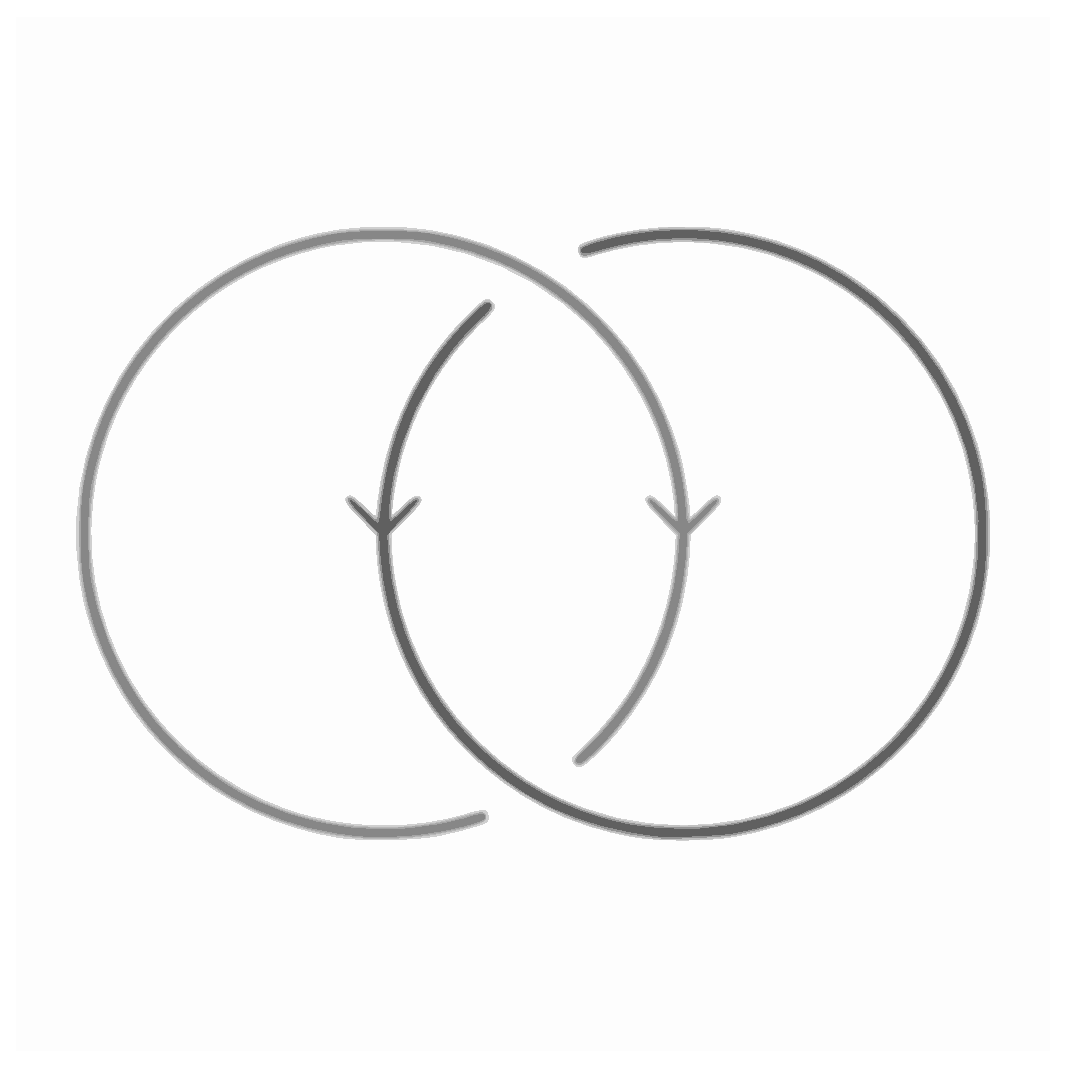
\includegraphics[width= 0.3\textwidth]{hopf}
            \caption{Die Hopf Verschlingung}
            \label{fig:hopf}
        \end{wrapfigure}
        Das trivialste nicht-triviale Beispiel einer Verschlingung mit mehreren Komponenten ist der Hopf Link. Er besteht aus zwei ineinander verschlungenen Unknoten, $L_1, L_2$. Betrachtet man nun zwei Scheiben und verklebt diese mit zwei umgekehrt verdrehten Bändern, so erhält man die Hopf Verschlingung als Rand. Äquivalent möge man sich einen Kreisring $S^1 \times I$ nehmen, der zweifach verdreht ist und beobachtet, dass dieser eine Seifertfläche $S$ darstellt. Das Geschlecht dieser Seifertfläche ist $0$, da es sich um eine Sphäre handelt, aus der zwei offene Scheiben entnommen wurde und somit $\chi_-(S)=0$. Mit anderen Worten ist die obige Bedingung, dass die Thurston-Norm eine Norm ist, nicht erfüllt. Entsprechend existieren Elemente in $H^1(M_L;\RR)$ die sich zu 0 auswerten und durch die Linearität der Thurston-Norm entsteht ein degenerierter Untervektorraum (man überprüft leicht, dass die Fortsetzung nach $\RR$ auch verschwindet). Mit der Subadditivität verschwindet die Thurston-Norm auf dem Vektorraum $H^1(M;\RR)$, also ist die Einheitskugel nicht kompakt, sondern der gesamte Raum. Geht man jedoch zur dualen Norm über, erhält man wieder ein kompaktes Polytop mit ganzzahligen Eckpunkten: 
        \[
              \overline B_{||\cdot||_T^*}= \{\alpha \in H_1(M;\RR)| \sup_{\{\phi \in H^1(M;\RR)\}} \phi(\alpha)\leq 1\}=0
        \] 

        Die folgenden Beispiele sind aus Thurston's Arbeit~\cite{Thurston.1986} entnommen. Die Berechnungen von Thurston bedienen sich lauter Argumente warum keine repräsentierende Fläche existieren kann, die eine geringere Komplexität als die bisher gefundenen hat. Wir werden natürlich unsere Anstrengungen belohnen und Theorem~\ref{thm:haupttheorem} nutzen, um die Thurston-Norm-minimierende Flächen bequemer festzustellen.

        \subsubsection*{Whitehead Verschlingung}

        Die Whitehead Verschlingung ist ein Link der aus zwei Komponenten $L_1,L_2$ besteht. Offensichtlich berandet jede Komponente $L_i$ in $M_{L_i}$ eine Scheibe, die sich in $M_L$ auf eine Kreisscheibe mit zwei entnommenen offenen Scheiben einschränkt (an den Stellen, an denen die offene Tubenumgebung des anderen Knotens die Scheibe durchdringt). Bei diesen Repräsentanten für $l_1$ beziehungsweise $l_2$ berechnet sich die Eulercharakteristik zu $-1$, also gilt $||\pm l_i||_T\leq 1$, offensichtlich gilt aber Gleichheit undin diesem Fall die Thurston-Norm eine tatsächliche Norm. Genauso offensichtlch gilt $||l_1+l_2||_T>0$: die Verschlingungszahl des Whitehead Links ist offensichtlich $0$ (dies sieht man indem man eine Projektion betrachtet in dem die eine Komponente der Unknoten ist), jedoch haben die Randkomponenten jeder Einbettung eines Kreisring $S^1\times I \into S^3$ Verschlingungszahl $\neq 0$ oder sind trivial (durch einen Äquator zu trennen). Also folgt, dass diese Fläche Geschlecht $\ge 1$ hat und somit $2 \leq ||l_1+l_2||_T \leq ||l_1||_T+||l_2||_T =2$ für eine Seifertfläche. Mit Theorem~\ref{thm:haupttheorem} ließe sich diese untere Abschätzung auch mit $\Delta_L = (L_1-1)(L_2-1) = L_1L_2 -L_1-L_2+1$ berechnen, da $\thur {l_1+l_2} \geq \alex {l_1+l_2} \geq (l_1+l_2) (L_1+L_2-0)=2$ Diese ist Seifert-Fläche ergibt sich sogar durch die Seifert-Konstruktion. Folglich:
        \begin{align*}
            ||l_1+l_2||_T =||-(l_1+l_2)||_T &\stackrel * = ||-l_1+l_2||_T = ||l_1-l_2||_T \\
            &=2
        \end{align*}
        wobei die ausgezeichnete Gleichung gilt, da $||-l_1+-l_2||_T\not \in \{0,1\}$ aus obigen Gründen.
        \emph{Behauptung:} Die Thurston-Norm Einheitskugel und ihr Duales sind die Folgenden:\\
        \begin{figure}[H]
        \centering
        \begin{subfigure}[l]{0.4\textwidth}
                \begin{tikzpicture}
            % Axis
            \draw[->] (-3,0)--(3,0) node[below] {$l_1$};
            \draw[->] (0,-3)--(0,3) node[left] {$l_2$};
        
            \draw[] (0,2)--(1,1);
            \draw[] (1,1)--(2,0);
            \draw[] (2,0)--(0,-2);
            \draw[] (0,-2)--(-2,0);
            \draw (-2,0)--(0,2);
        
            \node[below] at (2,0) {$l_2$};
            \node[above right] at (1,1) {$\frac {l_1+l_2}2$};
           % \filldraw[black] (1,1) circle (2pt) node[above right,black] {$\frac {l_1+l_2}2$};
            \foreach \Point in {(0,2), (1,1), (2,0), (0,-2), (-2,0), (0,2), (1,-1), (-1,-1),(-1,1)}{
            \node at \Point {\textbullet};
            }
        
            \end{tikzpicture}
                \caption{$\thurball$}\label{fig:whiteheadthur}
        
        
        \end{subfigure}    
        \hfill
    \begin{subfigure}[r]{0.4\textwidth}
              \begin{tikzpicture}
        % Axis
        \draw[->] (-3,0)--(3,0) node[below] {$L_1$};
        \draw[->] (0,-3)--(0,3) node[left] {$L_2$};

        \draw (-2, -2) --(-2, 0) --(-2, 2) --(0 ,2) --(2 ,2)--(2 ,0)--(2 ,-2) --(0 ,-2) --(-2,-2) ; 
        \foreach \Point in{(-2, -2) ,(-2, 0) ,(-2, 2) ,(0 ,-2) ,(0 ,2) ,(2 ,-2) ,(2 ,0) ,(2 ,2)}{
        \node at \Point {\textbullet};
        }
        \end{tikzpicture}
    \caption{$\dualthurball$}

    \end{subfigure}
    \caption{Einheitskugeln der Whitehead Verschlingung in $H^1(M;\RR)$ und $H_1(M;\RR)$}
    \end{figure}
    Die $8$ berechneten Punkte liegen auf dem Rand von $\thurball$ (die Norm ist stetig), einer konvexen Teilmenge. Es ist eine leichte Übung, dass jede konvexe Teilmenge zweier nächster Punkte in Abbildung~\ref{fig:whiteheadthur} im Rand dieser konvexen Teilmenge enthalten sein muss. Aufgrund der Monotonie folgt die Behauptung für die Einheitskugel. Für die duale Norm, berechnet man entweder $8$ verschiedene Randpunkte, oder beobachtet für jedes $\alpha \in H_1(M;\RR)$ auf welchen Elementen (eine Gerade) $\phi \in H^1(M_L;\RR)$ das Supremum $\phi \alpha$ angenommen wird und sieht direkt das Ergebnis.

    \subsubsection*{Borromäische Ringe}

    Seien $L=L_1 + L_2 + L_3$ die Borromäischen Ringe. Offensichtlich hat jede duale Fläche zu $l_i$, die Komponente $L_i$ als Rand, (sonst wäre der Meridian aufgrund eines Schnittzahlenarguments im Kern von $l_i$). Folglich hat also jede Fläche dual zu $l_i$ mindestens 3 Randkomponenten. Da eine Sphäre mit 3 entnommenen offenen Scheiben (also eine abgeschlossene Scheibe mit 2 Durchlöcherungen), wobei die eine Randkomponente aufgespannt wird von der entnommenen Komponente $\nu(L_i)$, bereits dual zu $l_i$ ist gilt wieder $\thur {\pm l_i}=1$ für jedes $i$. Ähnlich wie beim letzten Beispiel der Whitehead Verschlingungen, möchten wir nun --- in Dimension 3 --- die berandenden Seiten der Einheitskugel durch Berechnung einiger Punkte feststellen und sie dadurch bestimmen. Es berechnet sich $\Delta_L = L_1L_2L_3 -\sum L_iL_j + \sum L_i -1$ und somit folgt leicht die Alexander-Norm einer beliebigen Kohomologieklasse, insbesondere:
    \[
        3= \alex {\pm l_1 \pm l_2 \pm l_3} \leq \thur {\pm l_1 \pm l_2 \pm l_3} \leq  \thur {l_1} + \thur {l_2} + \thur{l_3}=3
    \]

    Wegen $\thur {\pm l_i} = 1$  und $\thur {\frac13(\pm l_1 \pm l_2 \pm l_3)}=1$ folgt dass die Randseiten der Einheitskugel, die Standard-2-Simplices sind, die von den Einheitsvektoren aufgespannt werden. Somit berechnet sich $\thurball$ zu einem Oktahedron, siehe Abbildung~\ref{fig:borromthur}. Mit derselben Überlegung wie im vorhergehenden Beispiel, erkennt man strahlenweise die Form von $\dualthurball$ als Würfel.

\begin{figure}
\centering
    \begin{subfigure}{0.4\textwidth}
    
        \tdplotsetmaincoords{70}{110}        
        \begin{tikzpicture}[tdplot_main_coords]

        \draw[dashed] (-2,0,0) -- (2,0,0) ;
        \draw[dashed] (0,-2,0) -- (0,2,0) ;
        \draw[dashed] (0,0,-2) -- (0,0,2); 
        \draw[->] (2,0,0) -- (3,0,0) node[anchor=north east]{$l_1$};
        \draw[->] (0,2,0) -- (0,3,0) node[anchor=north west]{$l_2$};
        \draw[->] (0,0,2) -- (0,0,3) node[anchor=south]{$l_3$};
    
    
        \foreach \x in {2,-2}{
                \node at (\x  ,0,0) {\textbullet};
                \node at (0,\x ,0) {\textbullet};
                \node at (0,0,\x ) {\textbullet};
                \draw (\x,0,0)--(0,\x,0);
                \draw (\x,0,0) -- (0,0,\x);
                \draw (\x,0,0)--(0,-\x,0);
                \draw (\x,0,0) -- (0,0,-\x);
                \draw (0,\x,0) -- (0,0,\x);
                \draw (0,\x,0) -- (0,0,-\x);
                }
            \draw [fill,opacity=0.3] (2,0,0) -- (0,2,0) -- (0,0,2) -- cycle;
         %   \draw[thick] (2/3-0.3,2/3,2/3) -- (2/3+0.3,2/3,2/3);
       %     \draw[thick] (2/3,2/3-0.2,2/3) -- (2/3,2/3+0.2,2/3);
         %   \draw[thick] (2/3,2/3,2/3-0.2) -- (2/3,2/3,2/3+0.2);
         %   \node[above] at (2/3+0.2,2/3,2/3+0.2) {$l/3$};
        \end{tikzpicture}
        \caption{$\thurball$}\label{fig:borromthur}
    \end{subfigure}
    \hfill
    \begin{subfigure}[r]{0.4\textwidth}
    
        \tdplotsetmaincoords{70}{110}
        \begin{tikzpicture}[tdplot_main_coords]

        \draw[dashed] (-2,0,0) -- (2,0,0) ;
        \draw[dashed] (0,-2,0) -- (0,2,0) ;
        \draw[dashed] (0,0,-2) -- (0,0,2); 
        \draw[->] (2,0,0) -- (3,0,0) node[anchor=north east]{$l_1$};
        \draw[->] (0,2,0) -- (0,3,0) node[anchor=north west]{$l_2$};
        \draw[->] (0,0,2) -- (0,0,3) node[anchor=south]{$l_3$};
    
        \foreach \x in {2,-2}{
                \node at (\x  ,0,0) {\textbullet};
                \node at (0,\x ,0) {\textbullet};
                \node at (0,0,\x ) {\textbullet};
                }
        \foreach \x in {2,-2}{
            \foreach \y in {2,-2}{
            \foreach \z in {2,-2}{
            \draw (\x,\y,\z) -- (\x,\y,-\z);
            \draw (\x,\y,\z) -- (-\x,\y,\z);
            \draw (\x,\y,\z) -- (\x,-\y,\z);
            }
            }
        }
        \end{tikzpicture}
        \caption{$\dualthurball$}
    \end{subfigure}
    \caption{Die Einheitskugeln der Borromäischen Ringe}
\end{figure}
